\documentclass[a4paper,10pt,landscape,twocolumn]{article}

\usepackage{préambule}
\usepackage{clipboard}
\usetikzlibrary{shapes,positioning}

\makeatletter
\renewcommand{\maketitle}{%
{\scriptsize colle dans ton cahier d'exercices}
	\begin{center}
		\LARGE
		\myuline{\@title}
		\vspace{0.5em}
	\end{center}
}
\makeatother

\title{Activité : pour s'échauffer}
\date{}
\author{}

\begin{document}

\Copy{Activité}{
	\maketitle

	Voici des relevé de températures d'un thermomètre en hiver :

	\begin{tikzpicture}[scale=0.4]
		\coordinate (Thermo1) at (0,0);
		\coordinate (Thermo2) at (10,0);
		\coordinate (Thermo3) at (20,0);

		\foreach \thermo \temp in {Thermo1/3,Thermo2/0,Thermo3/4} {
				\draw[rounded corners=2pt] (\thermo) ++(0,-6) rectangle ++(0.4,12);
				\foreach \t in {-5,-4,-3,-2,-1,0,1,2,3,4,5} {
						\draw (\thermo) ++(0.2,\t) -- ++(0.2,0);
					}
				\node at ([xshift=-1.2cm] \thermo) {\temp°C :};
				\draw[fill=black,rounded corners=2pt] (\thermo) ++(0,-6) rectangle ++(0.4,\directlua{tex.print(\temp + 6)});
			}
	\end{tikzpicture}

	\begin{enumerate}
		\item Écrit ces trois températures sur la figure ci-dessous. Quel est l'écart de température entre 2 graduations ?
		\item Dans la région où est placé le thermomètre, les températures descendent jusqu'à \textbf{-3°C}. Dessine le niveau du thermomètre dans ce cas.
		\item Sur chaque graduation, écrit la température qui correspond.
	\end{enumerate}


	\begin{center}
		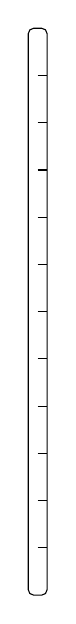
\begin{tikzpicture}[scale=0.6]
			\coordinate (Thermo) at (0,0);

			\draw[rounded corners=2pt] (Thermo) ++(0,-6) rectangle ++(0.4,12);
			\foreach \t in {-5,-4,-3,-2,-1,0,1,2,3,4,5} {
					\draw (Thermo) ++(0.2,\t) -- ++(0.2,0);
				}
		\end{tikzpicture}
	\end{center}
}

\Paste{Activité}

\end{document}